\documentclass[conference]{IEEEtran}
% Some Computer Society conferences also require the compsoc mode option,
% but others use the standard conference format.


% *** QUOTES PACKAGE ***
%\usepackage [english]{babel}
%\usepackage [autostyle, english = american]{csquotes}
%\MakeOuterQuote{”}

\usepackage[utf8]{inputenc}
\usepackage[T1]{fontenc}
\usepackage[threshold=1]{csquotes}


% *** GRAPHICS PACKAGE ***
\ifCLASSINFOpdf
  \usepackage[pdftex]{graphicx}
  % declare the path(s) where your graphic files are
  \graphicspath{{../images/}}
  % and their extensions so you won't have to specify these with
  % every instance of \includegraphics
  \DeclareGraphicsExtensions{.pdf,.jpeg,.png}
\else
  % or other class option (dvipsone, dvipdf, if not using dvips). graphicx
  % will default to the driver specified in the system graphics.cfg if no
  % driver is specified.
  \usepackage[dvips]{graphicx}
  % declare the path(s) where your graphic files are
  \graphicspath{{../images/}}
  % and their extensions so you won't have to specify these with
  % every instance of \includegraphics
  \DeclareGraphicsExtensions{.eps}
\fi

% correct bad hyphenation here
\hyphenation{op-tical net-works semi-conduc-tor}

\begin{document}

\title{Engineering Privacy and Protest:\\a Case Study of AdNauseam}

\author{
  \IEEEauthorblockN{Daniel C. Howe}
  \IEEEauthorblockA{School of Creative Media\\City University, Hong Kong\\Email: daniel@rednoise.org} \and
  \IEEEauthorblockN{Helen Nissenbaum}
  \IEEEauthorblockA{Cornell Tech\\New York University\\Email: hfn1@nyu.edu}
}

\maketitle

%\start{abstract}

\emph{Abstract}---The strategy of obfuscation has been broadly applied---in search, location tracking, private communication, anonymity---and, as such, has been recognized as an important element of the privacy engineer's toolbox. However, there remains a need for clearly articulated case studies describing not only the engineering of obfuscation mechanisms but, further, providing a critical appraisal of obfuscation's fit for specific socio-technical applications. This is the aim of our paper, which presents our experiences designing, implementing, and distributing AdNauseam, an open-source browser extension that leverages obfuscation to counter tracking by online advertisers.

At its core, AdNauseam works much like a list-based adblocker, hiding ads and blocking trackers. However, it provides two additional features. First, it collects each ad that it finds in its ‘Vault’, allowing users to interactively explore the ads they have been served, and providing insight into the algorithmic profiles created by advertising networks. Second, AdNauseam simulates clicks on each ad in order to confuse trackers and diminish the value of aggregated tracking data.

A critic might ask: why click? Why not simply hide ads from users and hide users from trackers? The twofold answer reveals what may be distinctive elements of the AdNauseam approach. To begin, we conceptualize privacy as a societal value. Whereas many privacy tools offer solutions only for individual users, AdNauseam is built on the assumption that, often, effective privacy protection must be infused throughout a system. This assumption presents different and interesting engineering challenges. Second, AdNauseam seeks to concurrently achieve the goal of resistance through protest. And since protest frequently involves being vocal, AdNauseam's core design at times conflicts with privacy conceptions based on secrecy and concealment. While such tensions, and the tradeoffs that result, are not uncommon in privacy engineering (for example, in private communications tools, between security properties and usability), the process of designing and building AdNauseam demanded their systematic consideration and resolution.

In this paper we describe the goals of the project, with a focus on the operational definition of privacy that serves as its guide, and the implemented features to which these goals map. We present the engineering approach employed, including tensions we encountered during implementation; how they were resolved and our methods of evaluation on both technical and ethical dimensions. We discuss challenges of distribution, including Google's ban of AdNauseam from its Chrome store. We conclude with thoughts on the broader challenges that face privacy tools which must operate within complex socio-technical contexts, especially those dominated by actors openly resistant to them.

%\end{abstract}
\vspace{5mm}

\begin{IEEEkeywords}
engineering, privacy, tracking, advertising, obfuscation, adblocking, surveillance, values-in-design
\end{IEEEkeywords}

% For peer review papers, you can put extra information on the cover page as needed:
% \ifCLASSOPTIONpeerreview
% \begin{center} \bfseries EDICS Category: 3-BBND \end{center}
% \fi
% For peerreview papers, this IEEEtran command inserts a page break and
% creates the second title. It will be ignored for other modes.
\IEEEpeerreviewmaketitle

\section{Introduction}

% no \IEEEPARstart
The ad blocking wars \cite{Nytimes} reflect wide ranging resistance to aspects of the online advertising landscape, specifically tracking, malware, annoyance, degradation of browser performance, and bandwidth costs. A number of technical systems, utilizing diverse techniques, have addressed these issues in various combinations. AdNauseam, an open-source, cross-platform browser extension, contributes to this growing arsenal not only by hiding ads and blocking malware, but by leveraging obfuscation to confound those seeking to profile users based on interests revealed through ad clicks. Specifically AdNauseam hides online ads while clicking each ad behind the scenes in order to register visits in ad network databases. The goal of the software is to pollute the data gathered by trackers and, by diminishing confidence in this particular indicator, render their efforts to profile less effective. At the same time, the software allows users to engage in a form of expression, by actively disrupting the economic system that drives surreptitious tracking, and by creating mistrust (advertisers generally pay ad networks for clicks) within the advertising system. Additionally, AdNauseam makes the ads it collects available to users to explore at their convenience, via multiple interactive displays designed to facilitate real-time understanding of the advertising system at work.


\subsection{Engineering Philosophy}

Our approach to the development of AdNauseam builds on prior work that has explicitly taken social values into consideration during tool design \cite{Friedman,Flanagan,Howe-1}. Throughout planning, development, and testing phases, we have integrated values-oriented concerns as first-order “constraints” together with more typical engineering metrics such as efficiency, speed, and robustness. Specific instances of values-oriented constraints include \emph{visibility and transparency} in interface, function, code, process, and strategy; \emph{personal autonomy}, where users need not rely on third parties; \emph{social protection of privacy} with distributed/community-oriented action; \emph{minimal resource consumption} (cognitive, bandwidth, client and server processing); and \emph{usability} (size, speed, configurability, ease-of-use). Enumerating values-oriented constraints early in the design process enables us to iteratively revisit and refine them in the context of specific technical decisions. Where relevant in the following sections, we discuss ways in which AdNauseam benefited from this values-oriented approach, as well as tensions between design goals that emerged. Additionally we have followed a number of strategies from the literature on privacy-by-design \cite{Gurses-0, Hoepman, Gurses-1, Hansen, Cavoukian} by including \emph{Data Minimization Strategies}, \emph{Legitimacy Analysis} and \emph{Socially-informed Risk Analysis} as elements of our design process.


\subsection{Design Goals and Constraints}

The AdNauseam extension is designed to realize three tangible goals for users, each of which addresses privacy in the context of online tracking via advertising. The first is to offer \emph{protection}; protection against malware and “malvertising” (malicious software that leverages advertising mechanisms to gain access to users' systems \cite{Mansfield}), as well as protection against data aggregation and data profiling via clicks on advertisements. The second goal is to provide a means of proactive engagement, allowing users an avenue for \emph{expression} of their dissatisfaction with current advertising mechanisms to those running the systems. In the case of AdNauseam, this expression has an interventional aspect, as the software actively attempts to disrupt the economic model that drives advertising surveillance. The third goal is to facilitate increased \emph{understanding} of the complex advertising ecosystem---and the profiling on which it operates---by providing users with the ability to view the ads they are served in real-time, and later, to explore interactive visualizations of the ads collected over time. These mechanisms are augmented by in-interface links to additional learning resources.


\subsection{Feature Mapping}

The mapping of goals to features (and to the system modules described below) was performed as follows: The goal of \emph{protection} was implemented at a basic level by the clicking of collected ads, via the visitation module; and by the blocking of non-visual trackers and malware, via the detection module. The former attempts to protect the user from data profiling via advertisements, and the latter from non-visual tracking and potential malware. \emph{Expression} was realized through clicks, again via the visitation module, and also in our implementation of the EFF's Do Not Track (DNT) mechanism \cite{EFF-1,EFF-2}. With DNT enabled (the default setting), the DNT header is sent with all requests, and ads on DNT sites remain visible. Ads on these DNT pages are also not visited by AdNauseam. The goal of increased \emph{understanding} is realized via in the visualization module, specifically via the real-time menu interface, where users can watch as new ads are discovered, then visited; the vault interface (descibed below), and a range of explanatory links embedded throughout AdNauseam's settings pages. Additionally, an in-depth Frequently-Asked-Questions (FAQ) list is linked from multiple locations within the interface, leading to over 40 carefully answered questions.


\subsection{Data Minimization}

Following a growing body of literature on privacy-by-design \cite{Gurses-0, Hoepman, Gurses-1, Hansen, Cavoukian}, our design and implementation process followed principles of data minimization. Thus AdNauseam was designed to function without ever communicating to a “home server” or sending user-data to any other entity, for any reason. Of course this means that, as developers, we are unable to access usage patterns and related data, which may have yielded important insights. Yet this a) clarified our own position in regard to privacy and data collection, and b) enabled us to sidestep potential problems of data leakage or interception in transit. Similarly, this principle helped us to identify three pieces of private information which could potentially be leaked during normal function of the tool, and to then expose these as user options, with defaults that would provide normal users with full protection, while allowing advanced users the option to change these settings for higher performance. These data were all potentially exposed to third-parties (websites and advertising networks) as part of the normal HTTP headers sent with requests for ads being clicked; specifically page referer, user-agent, and cookies. From either the referer or cookies, an advertising network present on multiple sites sites (Google, for example, is estimated to have code running on 70\% of websites \cite{Englehardt}) could potentially recreate large portions of a user's click path, while the user-agent header could be used by malicious trackers attempting to perform browser fingerprinting \cite{Nikiforakis}. Thus all such information was stripped from outgoing requests by default. As discussed below, this choice is not without consequences. Choosing to foreground the safety of user data in this way directly impacted AdNauseam's efficacy on other goals.

\vspace{2mm}
\blockquote{\emph{The application of data minimization does not necessarily imply anonymity, but may also be achieved by means of concealing information related to identifiable individuals} \cite{Gurses-0}.}
\vspace{1mm}

Additionally we have applied the principle of data minimization to our ad export feature, which allows users to export their aggregate ad collection (as JSON) in order to sync or migrate between machines, to backup, or to share. From our experiences user-testing this feature, we noted that such exports contained potentially sensitive data, specifically users' click trails (stored as the locations for found ads), possibly over months or even years. When considering how to handle this data we noted that it also existed in the browser's local storage, which could potentially be accessed by a malicious actor. Thus we subsequently implemented encryption for this data, both in memory and in storage, as well as offering the user the option, before each export, to redact all ad locations if desired.

\subsection{Legitimacy Analysis}

\vspace{1mm}
\blockquote{\emph{Before any privacy-by-design activities are embarked upon, a discussion needs to take place with respect to the “legitimacy” of the desired system given its burden on privacy. Legitimacy is described as “the establishment that the application goals would be useful for the intended use population” \cite{Iachello}. This question ought to also be re-iterated once the design of the system is completed, and possibly even after deployment} \cite{Gurses-1}.}
\vspace{1mm}

A critic might ask: why click? Why not simply hide ads from users and hide users from trackers? There are two reasons. First, AdNauseam is inspired by the path-breaking work of Priscilla Regan, who argued in her book, “Legislating Privacy”, that beyond its protection of individual interests, privacy serves social ends \cite{Regan}. In one version of this argument, privacy functions much like a collective good, such as clean air or national defense. As a non-excludable, indivisible collective good, privacy is not doled out individually. Although in certain situations it may be allocated according to individual needs and preferences, or even willingness to pay, and for these situations, privacy tools have been developed for individuals to use one-at-a-time. AdNauseam, however, embodies Regan's notion of privacy as a collective good. As such it fills the need of individual users, but also attempts to infuse privacy throughout a system. This commitment to privacy as a collective good presents different and interesting engineering and evaluation challenges, which, in our view, warrant close attention. Thus AdNauseam may stimulate deliberation not only on its particular architecture and features, but may draw attention to the conception of privacy it seeks to promote. A second reason for clicking, as opposed to simply blocking, is that AdNauseam seeks concurrently to achieve the goal of expressive resistance to tracking through protest. And since protest generally involves being vocal, AdNauseam's design seeks to give voice to users. It does not promote the conception of privacy as secrecy or concealment, as many other tools do, by enabling individuals to act stealthily and hide their tracks. Instead, it provides a means for users to express, in plain sight, their dissent by disrupting the dominant model of commercial surveillance.

Critics have warned that approaches such as AdNauseam's harm “independent content producers who can no longer support their sites.” As this critique touches a broad array of tools, including standard ad blockers, it will take us too far afield to address it in full here.  However, setting aside the rejoinder which points out that these sites are enabling surveillance, or more harshly, “selling out” their visitors, the hope is that loosening the chokehold of tracking over web and mobile domains will allow other business models to flourish. Toward this end we have enabled support in AdNauseam for the EFF's DNT mechanism, a machine-verifiable (and potentially legally-binding) assertion on the part of sites that commit to privacy-respecting behavior (for themselves and any third-parties present on their pages), at least for users who choose to send the DNT header \cite{EFF-1,EFF-2}. For sites that make this commitment, AdNauseam does not (by default) hide or block their ads or other resources, nor does it simulate clicks on their ads.

\subsection{Socially-informed Risk Analysis}

Given the goals we hoped to achieve and the set of features to which these mapped, we set out to identify risks to which users might be exposed. For each such risk, we considered the degree to which the user would be exposed when browsing the web using an unmodified browser, in comparison to the degree of exposure while using AdNauseam. Finally we considered their exposure using existing alternatives, ad-blockers like AdBlock Plus \cite{AdBlock} or wide-spectrum blockers like uBlock \cite{Gorhill}(see, for example, Figure \ref{fig:thirdparty} below). The following risks were identified:

\vspace{2mm}
\begin{itemize}
  \item Increased tracking by advertisers and other data-gatherers
  \item Personal data leakage (via clicks, via hiding rather than blocking, via ad export)
  \item Malware/malvertising
\end{itemize}
\vspace{2mm}

To establish a conservative lower-bound on exposure, we set a constraint on design and implementation decisions that user exposure with AdNauseam must be strictly lower on all dimensions than with our baseline case of browsing with an unmodified browser. Conversely, we hypothesized that the current performance of uBlock, the open-source blocker with the best performance metrics, would provide an upper-bound on risk exposure for the individual user. As AdNauseam must interact, at least minimally, with advertising servers in order to fulfill its functional requirements, it would necessarily expose users to more risk than the current state-of-the art blocker (e.g., uBlock), which does not have such a constraint. Notice that we refer specifically here to risk for \emph{the individual}, a distinction we return to below. In all cases (see \emph{Comparative Evaluation} below), we were able to verify that the risk to users on each of the dimensions listed above was strictly diminished by using AdNauseam, both in comparison to the no-blocker case, \emph{and} even in comparison to the most popular ad-blocker, AdBlock Plus \cite{PageFair}.


\subsection{Design Tensions}

\subsubsection{Indistinguishability and Data Leakage}

For obfuscation to function effectively as a means of counter-surveillance, the noise generated must exhibit a high degree of \emph{indistinguishability} with regards to data the system intends to capture; that is, it must be difficult for an adversary to distinguish injected noise from the data it is attempting to collect \cite{Gervais,Balsa}. Thus we strive to make AdNauseam visit requests indistinguishable from those sent for manual requests. However, there are  cases where this goal comes into tension with other aims of the software, specifically that of protection (both from malware and from data leakage). For example, when crafting a visit request, we must decide how accurately to mimic the data that the browser normally sends, specifically regarding user-agent and referer headers, and whether to include the cookies normally sent with the request. If we match these exactly then our request is indeed indistinguishable (assuming the browser is not modified to hide such details), and thus more difficult for an adversary to filter. However, this may also leak information to advertising networks that a user considers private, e.g., the URL of the page the ad was found on, the type of browser, operating system, etc. they are using. Similarly, we must decide whether to block incoming cookies from AdNauseam visits, whether the DOM of incoming request should be parsed and executed, and whether client-side scripts should be allowed to run.

While we can provide user configurable settings for all these parameters, we must still, for each case, consider the appropriate defaults by weighing risks to the user against potential gains in obfuscatory power (see \emph{Risk Analysis}). For AdNauseam, we have decided on default setting that maximize user protection. Thus, by default we block the user-agent header (to deter browser fingerprinting) and the referer (so as not to leak page-view data). Similarly, incoming cookies from visits are blocked---though this should not have any direct effect on indistinguishability---further minimizing the tracking to which users are exposed. Because visits are implemented via AJAX requests, a DOM is not constructed from the response and client-side scripts are not executed. While protection is maximized here, obfuscatory power may be diminished. For example, one vector of attack we have noted is from an adversary who, upon receiving a click request, sends a preliminary response containing JavaScript code that executes from within the DOM. In this case, if the client-side script never runs, then the click is never executed. We have experimented with solutions that address this issue and thus better support indistinguishability (including executing clicks in sandboxed invisible tabs), but have yet to find a solution that adequately protects user data and is cross-platform. For the moment we leave this as future work.

\vspace{1mm}
\blockquote{\emph{Cryptography researchers and privacy rights organizations tend to favor systems that prevent access to individuals and their information at all cost. The goal is to make access to the individual tamper-proof and to build a technological infrastructure based on nonidentifiability of users even vis-a-vis governments. Often, unfortunately, achieving this ambitious goal undermines system usability and drives system cost to a point where marketability and adoption of the solution becomes difficult} \cite{Spiekermann}.}
\vspace{1mm}

\subsubsection{Expression vs. Protection}

We have talked of the expressive and protective capabilities of data obfuscation generally, and of AdNauseam specifically. Abstractly conceived, these two capabilities seem to lie at opposite ends of a spectrum---on the one end, providing protection against surveillance and profiling, on the other, enabling users to be heard in their expressions of critique or protest. On the protective end, the noise generated by a system, as discussed above, must be indistinguishable. However, a tool that is perfectly protective (for which it is never possible to filter noise from data) will often be functionally invisible to an adversary. If an adversary is literally unaware of injected noise, then the expressive capability of that action is minimal (at least when considered from the perspective of the adversary). Conversely, if a system is highly expressive, it will likely be easier for an adversary to filter its noise, thus diminishing its protective capabilities. In the case of ScareMail (see \emph{Related Work} below), for example, it would be trivial for an engaged adversary to both detect users of the tool, and to filter out the noise generated by it. In practice, however, the relationship between expression and protection is more complex. Filtering might, in some cases, even serve to create temporary spaces free of surveillance. For example, in the case of ScareMail, an adversary filtering (and ignoring) data from ScareMail signatures might create a zone for messaging not subject to trigger-word monitoring, at least temporarily. A variation on this dynamic may affect AdNauseam users. Were an ad-network capable and willing to react by filtering AdNauseam clicks, users would be in the interesting position of being ignored by the system they are trying to evade. Being snubbed by the advertising system in this way means they will also have achieved the protection sought from AdNauseam.

The case of TrackMeNot \cite{Howe-2}, a tool that obfuscates users' interests in web search, also embodies subtle interactions between protection and expression. It is relatively easy for search engines to detect usage of the tool by referring due to the sudden spike in search frequency due to noise queries. Here, regardless of detection or filtering, users have already successfully communicated their discontent, possibly even forcing search engines to address the increase in resource usage. However, even if search engines know that users are employing TrackMeNot, they may not be able to perfectly distinguish between “real” and “fake” queries; that is, there may be some percentage of generated queries that are indistinguishable from user-generated queries (see \cite{Gervais} for an analysis of this question). As such, the tool provides expressiveness as well as a degree of protection. An adversary may be aware that a tool is injecting noise into its system, yet be technically, culturally, or otherwise unable or unwilling to filter it. From a tactical perspective, as tool designers leveraging obfuscation, this combination of protection and expression may be a sweet spot toward which we aim. To do so however will require more precise definitions of these criteria---how can we more formally evaluate, for example, the expressivity of a system that embeds complex interactions between human and non-human actors? We return to this question in our conclusions below.


\section{Architecture}

\subsection{Overview}

The AdNauseam software is comprised of four modules, each responsible for one of its primary functions: detection, extraction, visualization, and visitation.

\subsection{Detection}

This module is responsible for the analysis and categorization of requests following a page view. Such requests, most often to third-parties, is first classified according to the type of elements it realizes; whether advertisements, analytics, beacons, social-media, or functional widgets. The largest proportion of such requests (40-50\%) are made to the first group, on which this module focuses, which includes ad and ad tracking services \cite{Wills}. This module determines which requests to block and which to allow, and, in the latter category, between those that yield visual elements and those used only for tracking.

In order to categorize such requests, we leverage the capabilities of the open-source uBlock-Origin \cite{Gorhill} project, a configurable, list-based “blocker” that is effective and efficient \cite{Wills}. Like other blockers, uBlock allows users to specify publicly accessible lists of resources which contain syntactic matching rules for the retrieval of web resources. Based on these lists, we first determine whether a request should be blocked or allowed, and then, if allowed, whether it should be visible or hidden. If hidden, the element is downloaded and included in the page, but made invisible to the user via a content-script. Both blocking and hiding are specified via rules that may include the serving domain, the type of resource (e.g., images or video), and/or properties of the DOM container (for example, a DIV with a specific id or class). Rules are included from widely distributed lists that are updated and maintained by individuals and communities (e.g, “EasyList” \cite{EasyList}. Additionally, users can augment these lists with custom rules they create, either to block or hide new content, or to whitelist a page, site or element.

Requests marked as blockable in AdNauseam are disallowed at the network level, mimicing the behavior of most other blockers, including uBlock, AdBlock Plus, Adblock, and Adguard, which perform blocking on some percentage of requests and hiding on some percentage of the remainder. The difference for AdNauseam is that a subset of requests which might be blocked in other blockers must be allowed in AdNauseam; specifically those that result in, directly or indirectly, visual advertisements.\footnote{Interestingly, it is exactly this standard combination of functions---hiding and blocking---that Google cites as being in violation of its Terms of Service, a claim discussed below in the \emph{Distribution} section.} At the element hiding level, the detection module is invoked incrementally, via content-scripts, as page elements are loaded (or dynamically generated) and inserted into the DOM. Elements marked for hiding are assigned a CSS class that sets their display to invisible, and the surrounding DOM is collapsed so as not to leave blank space on the page. Each hidden element (generally a visual ad) is then passed to the \emph{Extraction} module.


\subsection{Extraction}

Once a visual element has been detected and hidden, we must then determine whether it is in fact an advertisement. If so, the extraction module of the system must extract the properties needed by the \emph{Visualization} and \emph{Visitation} modules. These properties include timestamp, size, content-url, target-url, page-detected-on, etc. Text-only ads, as often found on search engines, present a different challenge, as these are generally served inline along with page content rather than requested from a 3rd-party server. In these non-image cases, several additional fields are aggregated to form the content payload (title, description, tagline) and there is no content-url linking to an external resource. To enable extraction of such data, AdNauseam ships with a custom set of CSS selectors used to parse specific DOM attributes from text-ad sites (Google, Ask, Bing, etc.). Such filters run only on specific domains where text-ads have been previously discovered.


\subsection{Visualization}

In order to facilitate understanding online advertising systems, AdNauseam provides users with interactive visualizations of their collected ad data. These visualizations provide both high-level displays of aggregate data (see Figure \ref{fig:vault}), as well as the option to drill-down and inspect individual ads (see Figure \ref{fig:inspector}), for data fields including the page on which the ad was found, the target URL, the text copy, the viewed-on date, ad network, and image or video ‘content’. Additionally, a number of derived functions provide additional metrics (i.e., the total estimated charge to advertising networks for the ads visited on a given page or in a given time-period, as in Figure \ref{fig:menu}). Ads may be filtered and sorted according to a variety of criteria: by date, topic-category, ad-network, page-category, etc. The visualization module is a distinct contribution of AdNauseam, furthering our goal of increased understanding in two ways: 1) to enhance the user-experience with greater insight into the online advertising landscape; and 2) to enable interested users and researchers to study the ad data, and generate insight into the larger picture beyond momentary interactions. To facilitate these goals, we include mechanisms for importing and exporting ad data sets, which can be loaded and saved as plain-text JSON files directly from the extension. The use of this data, aggregated across users, for further research (with appropriate mechanisms for user consent) is an area we hope to explore in future work.

\begin{figure}[!t]
\centering
\includegraphics[width=2.5in]{images/vault.png}
\caption{AdNauseam's AdVault visualization.}
\label{fig:vault}
\vspace{10mm}
\includegraphics[width=2.5in]{images/inspector.png}
\caption{Inspecting a single ad in the AdVault.}
\label{fig:inspector}
\vspace{10mm}
\includegraphics[width=2.5in]{images/menu.png}
\caption{Estimated cost to advertising networks.}
\label{fig:menu}
\end{figure}


\subsection{Visitation}

This module simulates visits on collected ads, with the intention of appearing to the serving website (and the ad network) as if the ad had been manually clicked. Currently, these clicks are implemented via AJAX, which simulates requests (matching headers, referer, etc.) that the browser would normally send. This provides users with protection against potential malware in ad payloads, as responses are not executed in the browser, and JavaScript, Flash, and other client-side scripting mechanisms are not executed. Similarly, AdNauseam blocks incoming cookies for responses to ad visits. In making these design choices, we favored user-protection (from potentially dangerous ad payloads) to the appearance of authenticity in AdNauseam clicks, as discussed in the \emph{Design Tensions} section above.

What are the expected results of visiting some (or all) of users' collected ads? First, the data profiles of users stored by advertising networks and data brokers may be polluted, as users' actual interests are hidden by generated clicks. This both protects the individial user (assuming they have clicked or may click some ad in the future) as well as the larger user community, as aggregate statistics become less accurate. Second, as advertisers must now potentially pay publishers for decoy clicks, a degree of mistrust is introduced into the economic system. This is perhaps the most compelling argument for this strategy, as it could, given adequate adoption, force advertisers to change their behavior, either by developing new algorithms to filter such clicks, and/or by adopting more privacy-friendly policies (e.g., the EFF's DNT mechanism). However, AdNauseam's strategy has also attracted critics. Below we argue that this approach, although contentious, is ethically justified (at least while awaiting more long-term solutions) in order to protect users and safeguard privacy expectations. A more in-depth discussion of the ethical arguments related to visitation can be found in the \emph{Evaluation} section below.


\subsection{Distribution}

Although not often discussed in an engineering context, issues surrounding the distribution of AdNauseam highlight concerns we imagine will become only more relevant as corporate players exert a growing influence over the software ecosystem.

The prototype for AdNauseam was initially developed as a Firefox-only extension available in  Mozilla's addon store. In our production release, we added Opera and Chrome support and made the extension available in the Opera and Chrome stores respectively. We distributed upwards of 50,000 copies of the software over the subsequent six months, with the majority of these downloads coming from Google's Chrome store. On January 1, 2017 however, we learned that Google had banned AdNauseam from the store, and further, had begun disallowing even manual installation or updates of AdNauseam, effectively locking users out of their own saved data, all without prior notice or warning.

We wrote to Google requesting justification for the removal, and they responded that AdNauseam had breached the Web Stores Terms of Service, stating: “An extension should have a single purpose that is clear to users.”\footnote{In the one subsequent email we received, a Google representative stated that a single extension should not perform “both blocking and hiding,” an assertion that is difficult to accept at face value as nearly all ad blockers (including uBlock, AdBlock Plus, Adblock, Adguard, etc.) also perform blocking and hiding of ads, trackers, and malware, and have not thus far been banned. As of this writing in mid-February 2017, it has been over a month month since we have heard back from Google in response to our queries for clarification.} The single purpose of AdNauseam, we would argue, is not unclear at all---namely to resist the non-consensual surveillance conducted by advertising networks, of which Google is a prime example. Of course we understand that Google would prefer users not to install AdNauseam, as it opposes their core business model, but the Web Store's Terms of Service do not (at least thus far) require extensions to endorse Google's business model. Moreover, this is not the justification cited for the software's removal. Whether or not one is an advocate of obfuscation-based tools, it is disconcerting to know that Google can quietly make a privacy extension, along with stored data and preferences, disappear at any moment without warning. Here we see a counter-surveillance tool that is disabled; will tomorrow bring a secure chat app, or password manager? For developers, who, incidentally, must pay a fee to post items in the Chrome store, this should be a cause for concern. Not only can one's software be banned and removed without warning, but all comments, ratings, reviews, releases and statistics are deleted as well.


\section{Comparative Evaluation}

Qualitative Evaluation of AdNauseam was performed iteratively throughout development, often guided by solicited and unsolicited feedback from various constituencies, including users, developers, extension reviewers at Mozilla and the Opera store, and a range of privacy and security advocates. When considering how to evaluate the software, the question of whether AdNauseam in fact “worked” seemed at first to be the most obvious and simple to address. We soon realized, however, that the meaning of this question shifted as users' behaviors, goals, expectations, and perceived risks varied. Evaluating AdNauseam on the basis of feedback from the various constituencies was often a two-part process: first determining users' orientations, and then examining their feedback in light of their respective goals, concerns, and priorities. Additionally, beyond the technical issues with which we grappled, some of the critiques consistently expressed ethical concerns. Thus, we have split the evaluation discussion into two parts. The first focusing on technical considerations, the second on ethics.


\subsection{Technical}

Evaluation of obfuscation-based strategies for counter-surveillance is often a relatively straightforward challenge. As an example, consider the case of obfuscation in web search. To begin one might extract logs of queries from users, which contain both true queries and software-generated queries and run best-practice machine-learning (or other) algorithms to attempt to separate the two sets. Although one may never know the actual capabilities of an adversary (especially those, like Google, with vast resoures at their disposal), one can make educated guesses as to the type of attacks that might be performed, whether, for the search case, based on timing, query content, side-channels, or other means (for specific details of such evaluations in the search case, see \cite{Gervais,Balsa,Peddinti}).  If we find that the adversary can differentiate true queries with a high degree of accuracy, then the generated queries can be easily filtered  and, at least from a protection standpoint, the tool has failed.\footnote{We may still argue that the tool is successful in terms of expresssion, but this is a different concern.}

At first glance, evaluating AdNauseam seems similarly straightforward: to what degree of accuracy can an adversary, using state-of-the-art techniques, distinguish user clicks from AdNauseam-generated clicks? The question is confounded however by the fact that for the majority of users (those who enable the recommended ad hiding function and have disabled whitelisting for DNT sites), there are no true clicks to distinguish. No ads are seen, and thus none are ever clicked. At the same time, due to the frequency of clicks issued, an adversary will be able to readily ascertain that a user has installed AdNauseam. Given this information, we must ask what avenues are open to the adversary, whether technical or otherwise, and given these, what evaluation metrics might be applicable? One option is that all data for the user in question is discarded. From the user's perspective this may be considered a victory, as, at least in terms of clicks, they are no longer being profiled. However, since the data is discarded, there is also no net gain in privacy when considered from a communal perspective.

But what if the user does not hide all ads? Here there are two cases we must consider: the user who chooses to disable hiding altogether, and the user who selects a subset of ads to see, whether by whitelisting pages and sites by hand and/or by maintaining the default option to view ads from DNT-respecting sites. The former case, where a user goes through the trouble to install an adblocker, but continues to view all ads we imagine to be vanishingly small, so we focus on the latter, which consists of two sub-cases: the DNT case, and the non-DNT case. As DNT sites have made a binding commitment not to track users, protection is not needed, and generated clicks are thus not issued. In the user-whitelisting case, we find the situation that most closely the resembles the case of web search, where some subset of clicks are true and some generated. However the scenario is still different as here \emph{all} ads are clicked (the corollary would be if a user could issue all possible queries to a search engine). Thus for an adversary to distinguish true clicks, there must be some element of the click request itself on which to filter (the question of \emph{indistinguishability} discussed above). Thus we must verify that the formatting of our requests, including HTTP headers, cookies and other accompanying data, are identical for true and generated requests (Figure \ref{fig:headers} below). As such requests vary by browser, operating system, even by site, and may change over time (with or without action on the part of the adversary), this cannot be a one-time operation. Instead, we must test these values continuously (in the case of AdNauseam, we leverage an automated testing setup that tests a range of OS/browser/page combinations on a daily basis). Even if requests are indistinguishable, however, and the software is successful in frustrating filtering for passive adversaries, there a still side-channels available to a more determined adversary. One such attack is presented in the \emph{indistinguishability} section above.

\begin{figure}[!t]
\centering
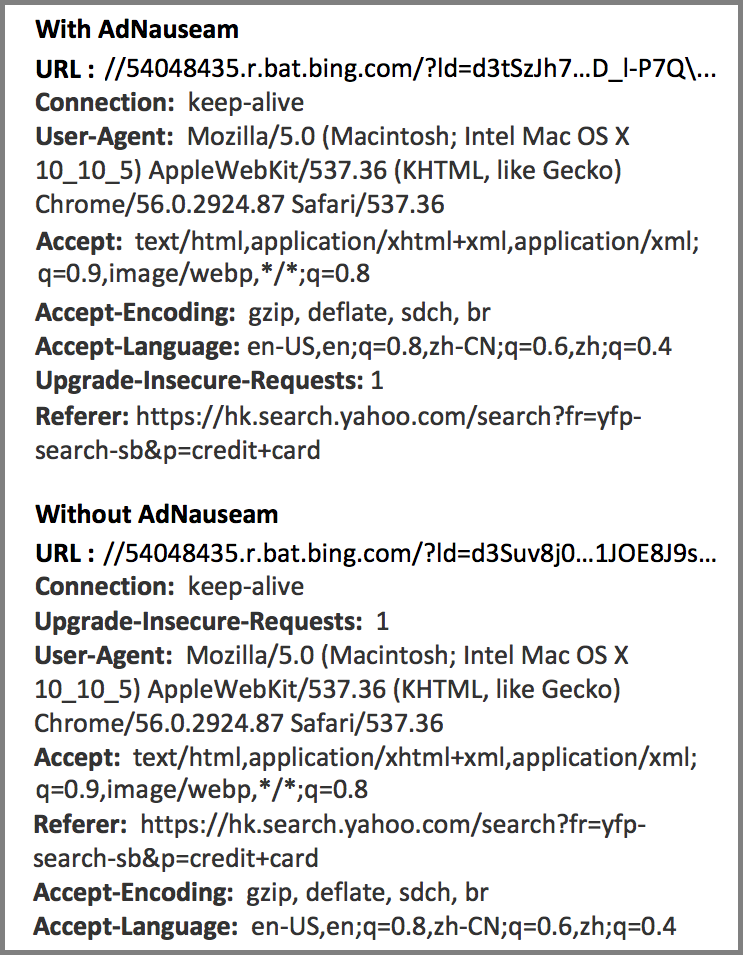
\includegraphics[width=2.5in]{images/headers.png}
\caption{Header Comparison: AdNauseam click vs. manual request}
\label{fig:headers}
\end{figure}

\subsubsection{Comparative Analysis}

To further evaluate the performance of AdNauseam, we compare it, on several dimensions (number of third-parties blocked, page load times, and memory use), to other browser extensions designed to protect users from online advertisers and trackers. Each test was first run without any extension, then with AdNauseam, then with Adblock Plus \cite{AdBlock}, currently the most widely installed adblocking extension, then with uBlock-Origin \cite{Gorhill}, the open-source content-blocker on which AdNauseam is based, and finally with Privacy Badger \cite{EFF-0}, discussed below in “Related Work”. Tests were performed using each extension's default settings after resetting the Chrome browser to its install state. After visiting each of the websites in the test set (between 15 and 85 popular URLS, depending on the test), via the Selenium browser automation tool, with each of the extensions, we evaluated their safety (Figure \ref{fig:thirdparty}) in terms of the number of 3rd parties interacted with, their memory efficiency (Figure \ref{fig:memory}), and their page-load speed (Figure \ref{fig:loadtime}). As shown in the graphs below, AdNauseam performed better on all dimensions than using either no blocker, or the highly popular AdBlock Plus. As expected, AdNauseam performed slightly less well than uBlock, due to the need to allow visual ad resources to download, rather than blocking them outright. Privacy Badger varied according to the specific test in question, as well as on whether it had been pre-trained before the test.

\begin{figure}[!t]
\centering
\includegraphics[width=2.5in]{images/thirdparty.png}
\caption{Number of distinct third-parties contacted.}
\label{fig:thirdparty}
\vspace{10mm}
\includegraphics[width=2.5in]{images/memory.png}
\caption{Overall memory footprint (MB).}
\label{fig:memory}
\vspace{10mm}
\includegraphics[width=2.5in]{images/loadtime.png}
\caption{Total page load time (sec).}
\label{fig:loadtime}
\end{figure}


\subsection{Ethical}

AdNauseam functions in a complex sociotechnical system, which is driven by political and economic motives hidden from ordinary users. Because most of us do not have the ability to influence or shape this system, interventions like AdNauseam (and others similar to it) provide a means of voicing discontent and achieving a cloak of protection. In the case of AdNauseam, the underlying mechanism is obfuscation---the deliberate and strategic injection of noise into technical systems in order to confound advertising trackers. In previous sections, we discussed known technical challenges and AdNauseam's attempts to meet them, but we also acknowledged that the limited, one-sided perspective of tool builders poses challenges to evaluation itself, that is, measuring the efficacy of selected mitigations. In spite of this, we have attempted to evaluate AdNauseam on various technical criteria and have compared its performance to other privacy-enhancing tools that address advertising. In this section, we focus on an equally important set of ethical challenges. AdNauseam invites two sources of ethical criticism. The first is concerned with its ad blocking function, the second with its data obfuscation function. Because ad blocking is neither distinctive nor (by design) AdNauseam's primary aim, and because it has already attracted significant public attention (e.g. the “ad block wars”), we set aside the active debates surrounding the use of ad blockers, resistance from service providers (recently Facebook \cite{Johnston}), and instead focus on whether the obfuscating strategy of clicking ads is defensible in ethical terms.

In adopting the philosophy of data obfuscation AdNauseam seeks to shields users from the inexorable, and inappropriate probes of services and third parties, not by hiding them from those parties but by transforming these probes into counter-probes (metaphorically, this philosophy resembles a judo master's---absorbing an attacker's energy to strengthen her own defensive counter strike). Choosing obfuscation, however, means taking seriously the ethical critiques that it has drawn, including charges that it is inherently dishonest, wastes resources, and pollutes data repositories, among others. Addressing these issues in \emph{Obfuscation: A User's Guide to Privacy and Protest} \cite{Brunton}, the authors charge creators of obfuscating systems to answer two questions: first, whether their aims are laudable; and second, whether alternative approaches exist which might achieve these aims at lesser cost. Because AdNauseam resembles other obfuscating systems discussed, its ethical legitimacy can be established for some of the features it shares with them. Given space limitations of this paper, we therefore focus on AdNauseam's distinctive features and the surrounding context relevant to its ethical evaluation.

Regarding Brunton and Nissenbaum's first charge, namely, ensuring that AdNauseam's aims are laudable, we take as a point of departure that ubiquitous online surveillance violates the tenets of a liberal democracy. The troubling nature of this surveillance apparatus is exacerbated by its surreptitious operation, its prevarication, and its resistance to the wishes of a majority of users. Others have eloquently established these claims through systems' analysis, demonstrations and public opinion surveys. \cite{Turow, Goldfarb, Malheiros, Tsai, Tucker} Data generated from online surveillance contributes to the creation of valuable, but often highly problematic profiles that fuel the information and behavioral advertising industries with uncertain, potentially negative effects on their subjects (for a good discussion, see \cite{Pasquale}). Against this backdrop, we judge the aims of AdNauseam, which include the disruption of this process, to be morally defensible.

The second charge to designers of obfuscating systems is whether the methods they have selected impose lower collateral costs than alternative approaches for achieving similar ends. Comparing the purported cost or damage caused by AdNauseam against alternative approaches involves more measurements and even more uncertainties than we are able to tackle here. But, by the same token, this dearth of concrete evidence also poses a challenge to critics who accuse ad blockers---and would similarly accuse AdNauseam---of harming the web's economy. Even if one holds that the “best” resolution would be societal-level regulation, there has been little progress on this front despite sustained privacy activism. Moreover, the promising beginnings of a multi-stakeholder solution, namely the Do-Not-Track initiative, was roundly scuttled by the online advertising industry. (For more information on this, see \cite{Brunton}.)
As important as seeking credible alternatives, however, is weighing the purported harms or costs of using AdNauseam. Among the latter, the harm of “wasting” network bandwidth or server resources is ironic at best, given the vast amount of bandwidth used by advertisers and trackers, the degradation in performance that results from loading this unwanted content into users' browsers, and the financial toll that such content takes on users paying for fixed data plans. From an ethical perspective, as argued in \emph{Obfuscation}, it is questionable whether the term “waste” is appropriate at all. We think not. For those who deliberately choose to install and use AdNauseam, it offers utility as a protective shield for privacy and an escape from inappropriate profiling. In our view, these are not worthless endeavors.

One of the most aggressive charges leveled at AdNauseam is that it perpetuates “click fraud.” Since obfuscation and fraud both involve forms of lying that disrupt entrenched systems, it is important to evaluate whether the two forms are alike.  To carry this out, we consult various definitions: “[Click] fraud occurs when a person, automated script or computer program imitates a legitimate user of a web browser, clicking on such an ad without having actual interest in the target of the ad's link” \cite{Liu} comes close to capturing AdNauseam in its notion of clicking without actual interest, but this definition seemed overly broad in that it commits users to click only on ads in which they are interested, and this seems an unjustifiable restriction on liberty of action. We also argue that if the automated script is performing as an agent of an individual, through that individual's legitimate choice, then the script is a proxy for the legitimate user. John Battelle's account \cite{Battelle}, which includes motive and intention, gets closer to the standard meaning of “fraud” in “click fraud”: the “‘decidedly black hat’ practice of publishers illegitimately gaming paid search advertising by employing robots or low-wage workers to repeatedly click on each AdSense ad on their sites, thereby generating money to be paid by the advertiser to the publisher and to Google.” Motivation is similarly important in this statement: “Click fraud is the subject of some controversy and increasing litigation due to the advertising networks being a key beneficiary of the fraud.” \cite{ClickFraud}
While elements of the above definitions ovelrap with AdNauseam's mechanized clicking on ads without genuine interest in their targets, machine automation is only incidental to click fraud, and may simply involve “low-wage workers.” More significant is what AdNauseam does not share with click fraud, namely action on behalf of stakeholders that serves either their direct financial interests or those of the developers or users of AdNauseam. In cases of click fraud that have been litigated, this condition, namely the intention to inflate earnings for those who employ them, has been critical. Finally, since we do not agree that visitors to websites have an obligation to click only those ads of genuine interest, we see no fraud in not doing so.

We readily admit that one of AdNauseam's primary aims in clicking all ads is to disrupt business models supporting surreptitious surveillance. From this, it does not follow however that AdNauseam (or other similar tools) is responsible for the demise of free content on the web. First, it is not, as we make clear on the project page, advertising itself that is the primary target of the project, but rather the ubiquitous tracking of users without their consent. Contextual advertising that does not involve tracking can certainly support free content just as it has in the past. Second, we should note that web content is not actually ‘free’ as this argument implies. The development of the Internet has been supported largely by government funding (and thus by taxpayers) since its beginning. In fact, vast infrastructure and energy costs are still born in large part by taxpayers, not to mention the potentially species-threatening cost to the environment posed by increasing data traffic \cite{Hazas}. Critics may say about users of AdNauseam, as they say about those who use ad blocking tools generally, that they free ride upon those who allow themselves to be tracked. However, in our view this presumes an entitlement on the part of trackers that is indefensible. Those who choose AdNauseam for its anti-profiling functionality may turn the tables on critics here, charging  trackers and profilers with destructive exploitation of users \cite{Brunton}. Lastly, in regard to free riding, we wish to point out that the hiding of ads is an optional element of AdNauseam, one that users must explicitly opt into when they install the software (see Figure \ref{fig:firstrun}); AdNauseam's visitation and visualization modules work equally well whether the user elects to view ads or to hide them.

\begin{figure}[!t]
\centering
\includegraphics[width=2.5in]{images/firstrun.png}
\caption{Opt-in sliders on first install page.}
\label{fig:firstrun}
\end{figure}


\section{Related Work}

The strategy of obfuscation has been broadly applied---in search \cite{Howe-2}, location tracking \cite{Meyerowitz}, social networks \cite{Luo}, anonymity \cite{Chakravarty, Schulze}, etc.---and, as such, has been recognized as an important element of the privacy engineer's toolbox. A range of obfuscation-based projects have been described in \cite{Brunton}, including FaceCloak \cite{Luo}, which obfuscates data profiles on the Facebook server, while the “true” profile is visible only to friends also using FaceCloak,  BitTorrent Hydra \cite{Schulze}, which encourages the proliferation of torrent sites to serve as decoys for anti-BitTorrent efforts, and CacheCloak \cite{Meyerowitz}, which sends GPS queries to mobile apps from diverse locations to mask users' actual locations. There have also been a number of obfuscation schemes for the web search case, five of which are detailed in Balsa et al \cite{Balsa}.

Other relevant work, described in \cite{Howe-3}, has come from the art/tech community. “I Like What I See” is a web browser extension that automatically clicks all ‘Like’ links on Facebook to obscure user interests. “ScareMail” \cite{Grosser}, mentioned above, is an extension built atop Gmail that append an algorithmically-generated narrative containing NSA “trigger-words” to the end of each composed email. “Invisible”\cite{Hagborg} extends obfuscation  to the terrestrial world of genetic privacy via a spray that obfuscates traces of DNA to frustrate identification.

Several user-level tools have been developed to address elements of advertising surveillance. Two earlier initiatives have attempted to provide ad-blocking integrated with some broadly-defined social good. AddArt \cite{AddArt} replaces blocked ads with user-configurable art, while AdLiPo \cite{Howe-0} replaces ads with constraint-based poetry, both offering playful alternatives to all-or-nothing ad blockers, while still providing relative awareness of ad content on pages. Lightbeam \cite{Mozilla} launched by Mozilla in 2013, provides displays of users' 3rd party connections when browsing the web, including advertising networks (though not advertisements themselves). Floodwatch \cite{Floodwatch}, described as “a collective ad-monitoring tool for social good,” is the one user tool of which we are aware that attempts to provide visualizations similar to our own, though it requires communication with a trusted 3rd-party server to do so; something at odds with our design goals. Privacy Badger \cite{EFF-0}, described as an extension that “blocks spying ads and invisible trackers” warrants mention in that it is the only other tool we have found that proposes a minimal avenue of resistance for users. The tool works to block third-party requests, but rather than operating via pre-compiled block lists, Privacy Badger makes real-time decisions based on content, blocking only those resources (ads included) which are engaged in tracking. Websites honoring the EFF's DNT header are whitelisted and no longer blocked, thus providing an incentive for content-providers to engage in privacy-respecting behavior. The current version of AdNauseam also includes this behavior (both the sending of the DNT header, and the whitelisting of sites who post their conformance to DNT).


\section{Future Work}

AdNauseam provides individuals with a means expressing a commitment to online privacy without the need to depend on the good will or intervention of third-parties. Although fully functional, AdNauseam is perhaps best considered as a proof of concept for a particular approach to privacy, that is, privacy through obfuscation. As discussed, AdNauseam's potential lies in its capacity to protect individuals against data profiling, as well as simultaneously providing a proactive means of expressing one's views to monolithic and largely uninterested corporations. One key challenge for AdNauseam and similar approaches is a means of providing rigorous, scientific assessments of performance against opaque adversaries; this is to say that we do not (and will not) know precisely the mechanisms that are in place for registering ad clicks, nor precisely the diverse interests of stakeholders in the online advertising ecology.

Going forward, a scientific approach to evaluating AdNauseam's performance, or the performance of any system adopting obfuscation, needs a means of measuring success---namely, evidence that decoy clicks have been registered and have an impact on the resulting profile. Such needs are likely to turn not only on the statistical analysis of signal-to-noise ratios, but also on a practical understanding of how ad-click data is actually mined and used, and the extent to which it influences aspects of user profiles. This would allow future iterations of obfuscation-based tools to be both effective and efficient in the noise they produce.

More concrete future work on AdNauseam could take several directions. In the near term we hope to better answer the question of how to perform indistinguishable clicks without leaking user data, as discussed above. Though complex, P2P approaches for the sharing of obfuscation data between users is a potentially ripe area of future work, and might also help address this issue, with users potentially visiting the ads detected by peers as a means of shielding their data, while maximizing the indistinguishability of visits. A central challenge here would be meeting functional criteria while not compromising the design constraints discussed early in this paper, e.g., transparency and independence from potentially untrustworthy third-parties.

\section{Conclusions}

AdNauseam operates in an environment that is both technologically and socially complex. Advertising mechanisms operate in a intricate, volatile, and competitive marketplace in which user data is percieved to be a highly valuable resource. For individuals, however, whether or not they view discrete online actions as sensitive, patterns recorded over time potentially open a window into their lives, interests, and ambitions. Thus the vast surveillance infrastructure that online advertising represents is not only a source of individual vulnerability, but also interferes with the rights to free and autonomous inquiry, association, and expression that are essential to a healthy democratic society, a distinction we explore above in our conception of privacy as a collective good. Consequently, there remain tensions between individual users, collective social and political values, and the economic interests of publishers and advertisers. In a better world, this tension would be resolved in a transparent, trust-based mutual accommodation of respective interests. Instead, users who are concerned with online privacy find little transparency and few credible assurances from advertisers that privacy will ever trump the pursuit of direct profit. In light of this, trust-based mutual accommodation of necessity gives way to an adversarial relationship, one in which we must, as privacy engineers, leverage all the strategies at our disposal, across the range of contexts in which privacy is threatened. Our success in this endeavor will depend in part on how well we share our experience applying known strategies to new contexts, in concrete and specific detail, according to an evolving set of best practices. This is what we have attempted to do above.

We conclude with a philosophical point.
 % concerning the legibility of human behavior to machinic systems.
In some of the most revealing exchanges we have had with critics, we note a palpable sense of indignation, one that appears to stem from the belief that human users have an \emph{obligation} to remain legible to their systems, a duty to remain trackable. We see things differently; advertisers and service providers are not by default entitled to the externalities of our online activity. Rather, average users should control the opacity of their actions, while powerful corporate entities should instead be held to high standards of transparency. Unfortunately this is the opposite of the status quo. The trackers want us to remain machine-readable, so that they can exploit our most human endeavors (sharing, learning, searching, socializing) to extract value and pursue profit. AdNauseam attempts to represent an alternative position.

\begin{thebibliography}{99}

\bibitem{AdBlock} AdBlock Plus. “AdBlock Plus.” n.d. https://adblockplus.org/.

\bibitem{AddArt} AddArt. “AddArt.” n.d. http://add-art.org/.

\bibitem{Balsa} Balsa, Ero, Carmela Troncoso, and Claudia Diaz. ``OB-PWS: Obfuscation-Based Private Web Search.'' \textbf{\textit{IEEE Symposium on Security and Privacy (SP)}}. IEEE, 2012.

\bibitem{Battelle} Battelle, John. \textbf{\textit{ The Search: How Google and Its Rivals Rewrote the Rules of Business and Transformed Our Culture}}. Nicholas Brealey Publishing, 2011.

\bibitem{Brunton} Brunton, Finn, and Helen Nissenbaum. \textbf{\textit{Obfuscation: A User's Guide for Privacy and Protest}}. MIT Press, 2015.

\bibitem{Cavoukian} Cavoukian, Ann, and Michelle Chibba. “Cognitive Cities, Big Data and Citizen Participation: The Essentials of Privacy and Security”. \textbf{\textit{Towards Cognitive Cities}}. Springer International Publishing, 2016. 61-82.

\bibitem{ClickFraud} Click Fraud. (n.d.). In Wikipedia. Retrieved August 1, 2016. https://en.wikipedia.org/wiki/Click\_fraud

\bibitem{Chakravarty} Chakravarty, Sambuddho, et al. “Detecting Traffic Snooping in Anonymity Networks Using Decoys.” (2011).

\bibitem{EasyList} “EasyList.” 2016. https://easylist.to/

\bibitem{Englehardt} Englehardt, Steven, and Arvind Narayanan. “Online Tracking: A 1-million-site Measurement and Analysis.” \textbf{\textit{Proceedings of the 2016 ACM SIGSAC Conference on Computer and Communications Security}}. ACM, 2016.

\bibitem{EFF-0} Electronic Frontier Foundation. “Privacy Badger.” n.d. https://www.eff.org/privacybadger.
\bibitem{EFF-1} Electronic Frontier Foundation. “Do Not Track.” n.d. https://www.eff.org/issues/do-not-track.
\bibitem{EFF-2} Electronic Frontier Foundation. “A privacy-friendly Do Not Track (DNT) Policy” n.d. https://www.eff.org/dnt-policy.

\bibitem{Flanagan} Flanagan, Mary, Daniel C. Howe, and Helen Nissenbaum. “Embodying Values in Technology: Theory and Practice.” \textbf{\textit{Information technology and moral philosophy}}. (2008): 322-353.

\bibitem{Floodwatch} Floodwatch. “FloodWatch.” n.d. https://floodwatch.o-c-r.org/.

\bibitem{Friedman} Friedman, Batya, Daniel C. Howe, and Edward Felten. “Informed Consent in the Mozilla Browser: Implementing Value-Sensitive Design”. \textbf{\textit{Proceedings of the 35th Annual Hawaii International Conference on System Sciences}}. IEEE, 2002.

\bibitem{Gervais} Gervais, Arthur, et al. “Quantifying Web-Search Privacy.” \textbf{\textit{Proceedings of the 2014 ACM SIGSAC Conference on Computer and Communications Security}}. ACM, 2014.

\bibitem{Goldfarb} Goldfarb, Avi, and Catherine Tucker. “Shifts in Privacy Concerns.” \textbf{\textit{The American Economic Review}} 102.3 (2012): 349-353.

\bibitem{Gorhill} Gorhill. “uBlock Origin - An efficient blocker for Chromium and Firefox.” 2016. https://github.com/gorhill/uBlock

\bibitem{Grosser} Grosser, Ben. “ScareMail.” 2013.\\ Web http://bengrosser.com/projects/scaremail/.

\bibitem{Gurses-0} G\"urses, Seda, Carmela Troncoso, and Claudia Diaz. “Engineering Privacy by Design.” \textbf{\textit{Computers, Privacy \& Data Protection}} 14.3 (2011).

\bibitem{Gurses-1} G\"urses, Seda, Carmela Troncoso, and Claudia Diaz. “Engineering Privacy by Design Reloaded.” \textbf{\textit{Amsterdam Privacy Conference}}. 2015.

\bibitem{Hagborg} Dewey-Hagborg, H. ``Invisible.'' 2014. \\ http://www.newmuseumstore.org/browse.cfm/invisible/4,6471.html.

\bibitem{Hansen} Hansen, Marit, Meiko Jensen, and Martin Rost. “Protection Goals for Privacy Engineering.” \textbf{\textit{Security and Privacy Workshops (SPW)}}. IEEE, 2015.

\bibitem{Hazas} Hazas, Mike, et al. “Are there limits to growth in data traffic?: On time use, data generation and speed.” \textbf{\textit{Proceedings of the Second Workshop on Computing within Limits}}. ACM, 2016.

\bibitem{Hoepman} Hoepman, Jaap-Henk. “Privacy Design Strategies.” \textbf{\textit{IFIP International Information Security Conference}}. Springer Berlin Heidelberg, 2014.

\bibitem{Howe-0} Howe, Daniel C. “AdLiPo” 2014. http://rednoise.org/adlipo/.

\bibitem{Howe-1} Howe, Daniel C. and Helen Nissenbaum. “TrackMeNot: Resisting Surveillance in Web Search.” \textbf{\textit{Lessons from the Identity Trail: Anonymity, Privacy and Identity in a Networked Society}} 23 (2009): 417-436.

\bibitem{Howe-2} Howe, Daniel C. and Nissenbaum, Helen. “TrackMeNot” New York University Computer Science Aug. 2006. Software/browser extension http://cs.nyu.edu/trackmenot/

\bibitem{Howe-3} Howe, Daniel C. “Surveillance Countermeasures: Expressive Privacy via Obfuscation”. APRJA, A Peer-Reviewed Journal About Datafied Research 4.1 (2015).

\bibitem{Iachello} Iachello, Giovanni, and Gregory D. Abowd. “Privacy and Proportionality: Adapting Legal Evaluation Techniques to Inform Design In Ubiquitous Computing.” \textbf{\textit{Proceedings of the SIGCHI conference on Human factors in computing systems}}. ACM, 2005.

\bibitem{Johnston} Johnston, Casey. “Why Facebook Is Really Blocking the Ad Blockers” \textbf{\textit{The New Yorker}}, 12 Aug. 2016.

\bibitem{Liu} Liu, De, Jianqing Chen, and Andrew B. Whinston. “Current Issues in Keyword Auctions”. \textbf{\textit{Business Computing (Handbooks in Information Systems, Vol. 3)}} (2009): 69-97.

\bibitem{Luo} Luo, Wanying, Qi Xie, and Urs Hengartner. “FaceCloak: An Architecture for User Privacy on Social Networking Sites” \textbf{\textit{International Conference on Computational Science and Engineering}}, 2009.

\bibitem{Malheiros} Malheiros, Miguel, et al.“Too close for comfort: A study of the effectiveness and acceptability of rich-media personalized advertising”. \textbf{\textit{Proceedings of the SIGCHI conference on human factors in computing systems}}. ACM, 2012. (pp. 579–588).

\bibitem{Mansfield} Mansfield-Devine, Steve. “When advertising turns nasty”. \textbf{\textit{Network Security}} 2015.11 (2015): 5-8.

\bibitem{Meyerowitz} Meyerowitz, Joseph and Romit Roy Choudhury. “Hiding stars with fireworks: Location privacy through camouflage.” \textbf{\textit{Proceedings of the 15th annual international conference on Mobile computing and networking}}. ACM, 2009.

\bibitem{Mozilla} Mozilla. “LightBeam.” 2016. https://www.mozilla.org/en-US/lightbeam/.

\bibitem{Nytimes} Murphy, Kate. “The Ad Blocking Wars.” \textbf{\textit{The New York Times}}, 20 Feb. 2016.

\bibitem{Nikiforakis} Nikiforakis, Nick, et al. “Cookieless monster: Exploring the ecosystem of web-based device fingerprinting.” \textbf{\textit{IEEE symposium on Security and privacy (SP)}}. IEEE, 2013.

\bibitem{PageFair} PageFair, Adobe “The cost of ad blocking–PageFair and Adobe 2015 Ad Blocking Report (2015).”

\bibitem{Pasquale} Pasquale, Frank. \textbf{\textit{The black box society: The secret algorithms that control money and information.}} Harvard University Press, 2015.

\bibitem{Peddinti} Peddinti, Sai Teja, and Nitesh Saxena. “On the Privacy of Web Search Based on Query
Obfuscation: A Case Study of TrackMeNot.” \textbf{\textit{International Symposium on Privacy Enhancing Technologies Symposium}}. Springer Berlin Heidelberg, 2010.

\bibitem{Regan} Regan, Priscilla M. \textbf{\textit{Legislating privacy: Technology, social values, and public policy.}} Univ of North Carolina Press, 1995.

\bibitem{Schulze} Schulze, Hendrik, and Klaus Mochalski. “Internet Study 2008/2009.” \textbf{\textit{Ipoque Report}} 37 (2009): 351-362.

\bibitem{Spiekermann} Spiekermann, Sarah, and Lorrie Faith Cranor. “Engineering Privacy.” \textbf{\textit{IEEE Transactions on software engineering}} 35.1 (2009): 67-82.

\bibitem{Tsai} Tsai, Janice Y., et al. “The effect of online privacy information on purchasing behavior: An experimental study.” \textbf{\textit{Information Systems Research}} 22.2 (2011): 254-268.

\bibitem{Tucker} Tucker, Catherine E. “Social networks, personalized advertising, and privacy controls.” \textbf{\textit{Journal of Marketing Research}} 51.5 (2014): 546-562.

\bibitem{Turow} Turow, Joseph, et al. “Americans reject tailored advertising and three activities that enable it.” (2009).

\bibitem{Wills} Wills, Craig E., and Doruk C. Uzunoglu. “What Ad Blockers Are (and Are Not) Doing." \textbf{\textit{Fourth IEEE Workshop on Hot Topics in Web Systems and Technologies (HotWeb)}}. IEEE, 2016.


\end{thebibliography}

\end{document}
